
\definecolor{codegreen}{rgb}{0,0.6,0}
\definecolor{codegray}{rgb}{0.5,0.5,0.5}
\definecolor{codepurple}{rgb}{0.58,0,0.82}
\definecolor{backcolour}{rgb}{0.95,0.95,0.92}

\lstdefinestyle{mystyle}{
	backgroundcolor=\color{backcolour},   
	commentstyle=\color{codegreen},
	keywordstyle=\color{magenta},
	numberstyle=\tiny\color{codegray},
	stringstyle=\color{codepurple},
	basicstyle=\ttfamily\footnotesize,
	breakatwhitespace=false,         
	breaklines=true,                 
	captionpos=b,                    
	keepspaces=true,                 
	numbers=left,                    
	numbersep=5pt,                  
	showspaces=false,                
	showstringspaces=false,
	showtabs=false,                  
	tabsize=2
}

\lstset{style=mystyle}

\section{intro til data }
To determine whether the data set meets the assumption of homoscedasticity, a scatter plot between the dependent and independent variables is created. It becomes apparent that the variables displacement, weight, and acceleration are not homoscedastic.Furthermore, MPG, displacement, weight, and acceleration are continuous numeric variables, while cylinders, model year, and origin are discrete numeric variables. Additionally, a heat map of the correlation between variables is created to determine if multicollinearity is present among the independent variables. Here, it is apparent that weight, displacement, and cylinders are highly correlated, and that all three are highly correlated with MPG. It is also clear from observing the density functions of the independent variables that none of them, except acceleration, are normally distributed. 
\lstinputlisting[language=R, caption=intro til data]{C:/Users/Jonathan/Documents/GitHub/P2/R kode/intro.R}



\begin{figure}[h] 
	\centering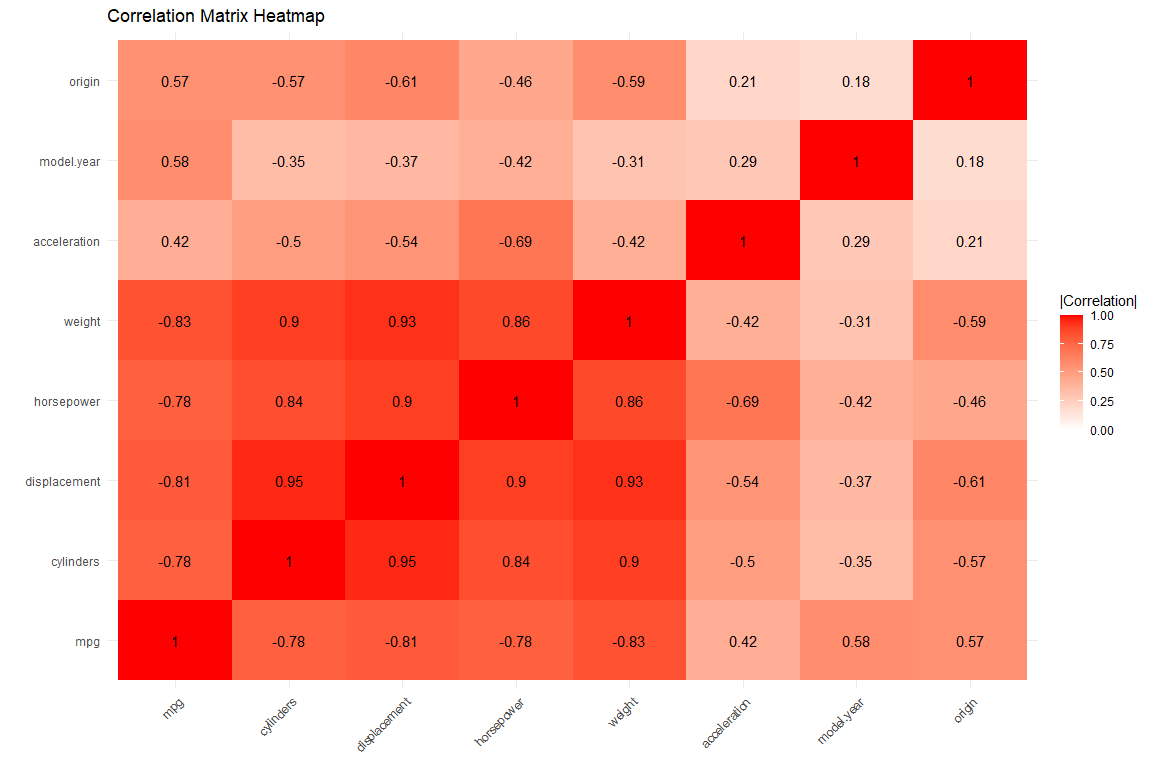
\includegraphics[width=14cm]{p2/1.png}
	\caption{heatmap}
	\label{fig:intro1}
\end{figure}


\begin{figure}[h] 
	\centering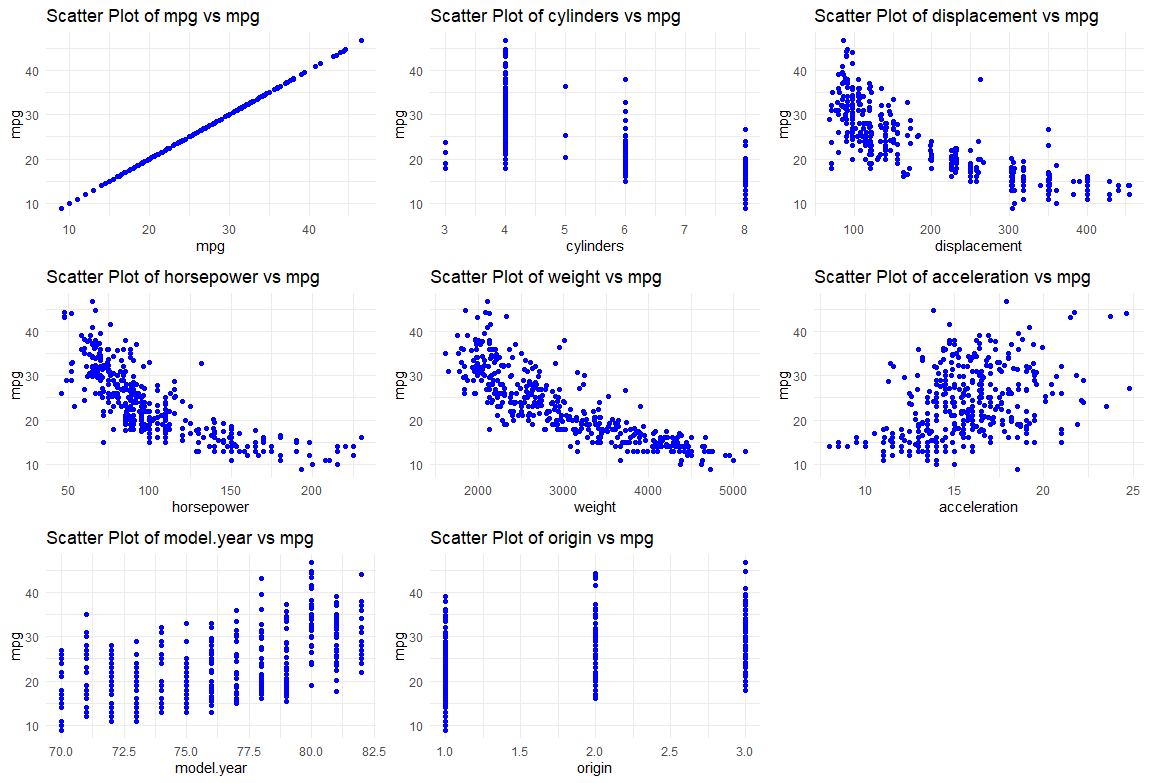
\includegraphics[width=14cm]{p2/2.png}
	\caption{scatterplot}
	\label{fig:instro2}
\end{figure}

\begin{figure}[h] 
	\centering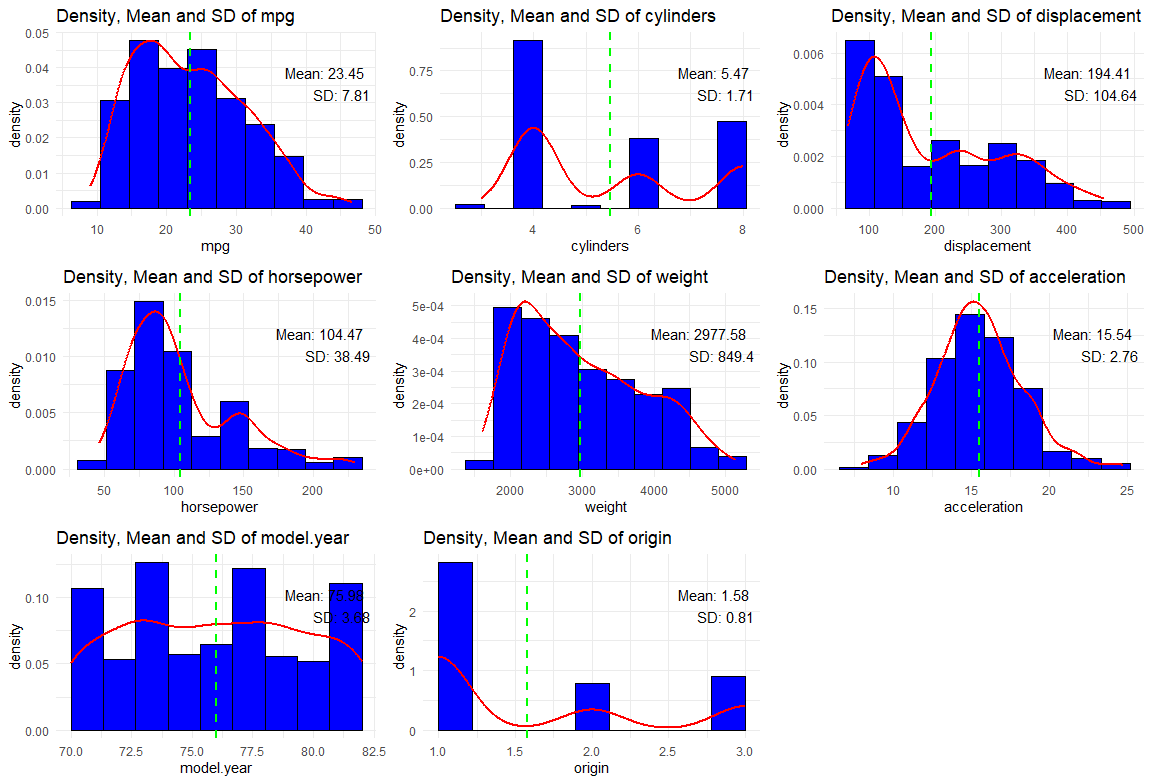
\includegraphics[width=14cm]{p2/3.png}
	\caption{density,mean and sd}
	\label{fig:intro3}
\end{figure}